\documentclass{standalone}
\usepackage{bm}
\usepackage{xcolor}
\usepackage{tikz}
\usetikzlibrary{decorations.pathmorphing, shapes.misc, calc}

\definecolor{mLightBrown}{HTML}{EB811B}
\definecolor{mLightGreen}{HTML}{14B03D}
\def\baselen{2.6cm}

\begin{document}

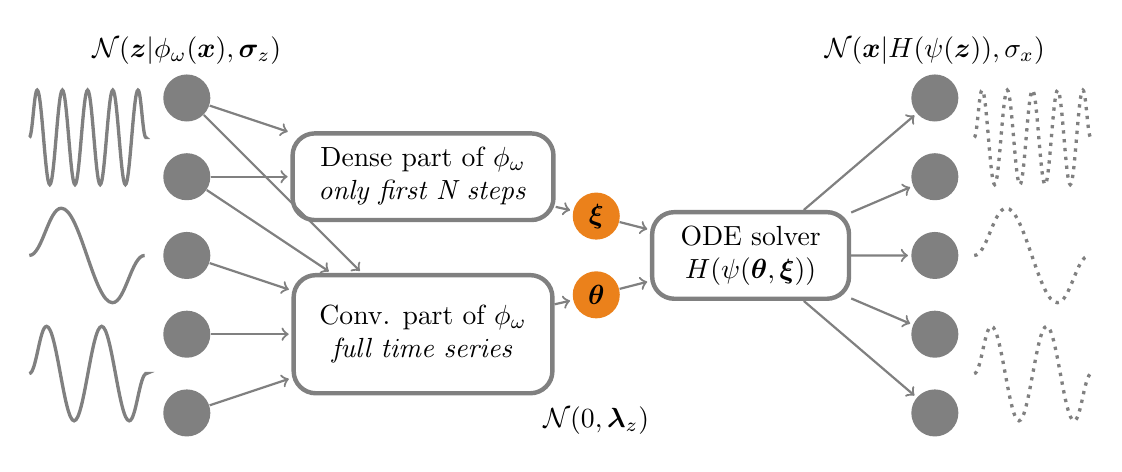
\begin{tikzpicture}[shorten >=1pt,->,draw=black!50, node distance=\baselen]
  \tikzstyle{every pin edge}=[<-,shorten <=1pt]
  \tikzstyle{neuron}=[circle,fill=black!25,minimum size=17pt,inner sep=0pt]
  \tikzstyle{input neuron}=[neuron, fill=gray];
  \tikzstyle{output neuron}=[neuron, fill=gray];
  \tikzstyle{hidden neuron}=[neuron, fill=mLightBrown];
  \tikzstyle{annot} = [text width=4em, text centered]

  % Draw the input layer nodes
  \foreach \name / \y in {1,...,5}
  % This is the same as writing \foreach \name / \y in {1/1,2/2,3/3,4/4}
    \node[input neuron] (I-\name) at (-3,-\y) {};

  \node[draw, ultra thick, rounded corners=8, minimum width=\baselen, minimum height=1.1cm]
    (dense) at ($(I-2) + (3,0)$) {
      \begin{tabular}{c}
        Dense part of $\phi_\omega$ \\ \emph{only first N steps}
      \end{tabular}
    };
  \node[draw, ultra thick, rounded corners=8, minimum width=\baselen, minimum height=1.5cm]
    (conv) at ($(I-4) + (3,0)$) {
      \begin{tabular}{c}
        Conv. part of $\phi_\omega$\\
        \emph{full time series}
      \end{tabular}
    };

  % Draw the hidden layer nodes
  \node[hidden neuron] (H-1) at (2.2cm,-2.5cm) {$\bm \xi$};
  \node[hidden neuron] (H-2) at (2.2cm,-3.5cm) {$\bm \theta$};

  % Connect input -> conv
  \foreach \source in {1,...,5}
    \path[thick] (I-\source) edge (conv);
  % Connect input -> dense
  \path[thick] (I-1) edge (dense);
  \path[thick] (I-2) edge (dense);

  % Connect networks -> latent
  \path[thick] (dense) edge (H-1);
  \path[thick] (conv) edge (H-2);

  % Draw the output layer nodes
  \foreach \name / \y in {1,...,5}
      \node[output neuron] (O-\name) at (\baselen*2.5,-\y cm) {};

  % draw and connect decoder
  \node[draw, ultra thick, rounded corners=8, minimum height=1.1cm, minimum width=2.5cm]
      (odesolve) at  (\baselen*1.6, -3) {
        \begin{tabular}{c}
          ODE solver\\
          $H(\psi(\bm \theta, \bm \xi))$
        \end{tabular}
      };
  \foreach \name / \y in {1,...,2}
      \path[thick] (H-\name) edge (odesolve);
  \foreach \dest in {1,...,5}
      \path[thick] (odesolve) edge (O-\dest);

  % input sines
  \draw[-, very thick, decoration={snake, segment length=0.32cm, amplitude=0.6cm}, decorate]
    ($(I-1) - (2, .5)$) -- ($(I-1) - (.5, .5)$);
  \draw[-, very thick, decoration={snake, segment length=1.3cm, amplitude=0.6cm}, decorate]
    ($(I-1) - (2, 2)$) -- ($(I-1) - (.5, 2)$);
  \draw[-, very thick, decoration={snake, segment length=0.7cm, amplitude=0.6cm}, decorate]
    ($(I-1) - (2, 3.5)$) -- ($(I-1) - (.5, 3.5)$);

  % output sines
  \draw[-,dotted, very thick, decoration={snake, segment length=0.32cm, amplitude=0.6cm}, decorate]
    ($(O-1) + (.5, -.5)$)--($(O-1) + (2, -.5)$);
  \draw[-,dotted, very thick, decoration={snake, segment length=1.3cm, amplitude=0.6cm}, decorate]
    ($(O-1) + (.5, -2)$)--($(O-1) + (2, -2)$);
  \draw[-,dotted, very thick, decoration={snake, segment length=0.7cm, amplitude=0.6cm}, decorate]
    ($(O-1) + (.5, -3.5)$)--($(O-1) + (2, -3.5)$);


  % Annotate with distributions
  \node[above of=I-3] (pzx) {$\mathcal{N}(\bm z | \phi_\omega(\bm x), \bm\sigma_z)$};
  \node[annot, below of=H-1] (pzx) {$\mathcal{N}(0, \bm \lambda_z)$};
  \node[above of=O-3] (pxz) {$\mathcal{N}(\bm x | H(\psi(\bm z)), \sigma_x)$};
\end{tikzpicture}

\end{document}
